% This is samplepaper.tex, a sample chapter demonstrating the
% LLNCS macro package for Springer Computer Science proceedings;
% Version 2.21 of 2022/01/12
%
\documentclass[runningheads]{llncs}
%
\usepackage[T1]{fontenc}
\usepackage{enumitem,amssymb}
\usepackage{amsmath} 
\usepackage{booktabs}

\newlist{todolist}{itemize}{2}
\setlist[todolist]{label=$\square$}
% T1 fonts will be used to generate the final print and online PDFs,
% so please use T1 fonts in your manuscript whenever possible.
% Other font encondings may result in incorrect characters.
%
\usepackage{graphicx}
% Used for displaying a sample figure. If possible, figure files should
% be included in EPS format.
\usepackage{hyperref}
% If you use the hyperref package, please uncomment the following two lines
% to display URLs in blue roman font according to Springer's eBook style:
\usepackage{color}
\renewcommand\UrlFont{\color{blue}\rmfamily}
% \urlstyle{rm}
%

\input{reviewing}

\begin{document}
%
\title{Benchmarking User-Specific Link Traversal Query Optimization: Evidence-Based Simulation of Decentralized Query Patterns } 
\rt{Since this is a resource paper, I'd recommend giving your benchmark/simulator a name. Maybe some word-play around users and SolidBench. U-SolidBench? MySolidBench? SolidBenchU? ... A title could then become something in the form of "SolidBenchU: Evidence-Based Simulation Benchmark for User-Specific Queries within Decentralized Environments"}
\author{Ruben Eschauzier\inst{1}\orcidID{0000-0002-6475-806X} \and
Ruben Taelman\inst{1}\orcidID{0000-0001-5118-256X}}

\institute{Department of Electronics and Information Systems, Ghent University – imec}
\titlerunning{Revisiting Link Prioritization for Efficient Traversal}

%
% \authorrunning{F. Author et al.}
% First names are abbreviated in the running head.
% If there are more than two authors, 'et al.' is used.
%
% \email{lncs@springer.com}\\
% \url{http://www.springer.com/gp/computer-science/lncs} \and
% ABC Institute, Rupert-Karls-University Heidelberg, Heidelberg, Germany\\
%
\maketitle              % typeset the header of the contribution
%
\begin{abstract}
% Context:      Why the need is so pressing or important
Optimizing queries in decentralized environments, 
where data sources are often unknown and dynamically discovered, 
remains a major challenge due to the lack of prior knowledge about data distribution and availability.
\rt{I would add one sentence here (or otherwise incorporate it above) to motivate the need for user-specific client-side query engines. Something like: Client-side apps can reuse the same client-side query engine, which introduces optimization opportunities.}
% Need:         Why something needed to be done at all
User-specific client-side query engines can mitigate this limitation by exploiting patterns in previously issued queries.
However, existing benchmarks fail to accurately reflect the performance \rt{Not sure "performance" is the right word here. I would talk about the typical properties and characteristics of user-specificness, or something like that, which then can lead to better performance.} of such approaches,
as they typically rely on repetitive or template-based query structures that lack realistic variability.
Moreover, publicly available query logs from real decentralized applications are scarce or absent in the literature.
Consequently, the evaluation of client-side decentralized query optimization techniques remains incomplete and cannot be performed under representative conditions.
% Task:         What was undertaken to address the need
To fill this gap, we introduce an evidence-based simulation of client query usage patterns \rt{... and offer it as a reusable benchmark(?)}.
This simulation \rt{benchmark?} enables systematic evaluation and comparison of client-side optimization techniques under realistic and reproducible conditions.
% Object:       What the present document does or covers
We demonstrate its use by applying it to a novel caching-based link traversal query processing approach.
To assess the impact of realistic query sequences, we compare the results against a benchmark that is not sequence-based, 
highlighting how query sequence simulation influences client-side optimization performance.
% Findings:     What the work done yielded or revealed
We find that [placeholder for results].
% Conclusion:   What the findings mean for the audience
We conclude: [placeholder for conclusion]

\keywords{First keyword  \and Second keyword \and Another keyword.}
\end{abstract}


% \section{TODO For Final Experiment}
%   \begin{todolist}
%     \item Investigate why the medium cache has a calculatedSize of 350000 in evictions.
%   \end{todolist}
% \textbf{Planned figures:}
% \begin{todolist}
%     \item unindexed-cache, indexed-cache, estimate-indexed-cache cactus plot
%     \item (Optional) Correlation between cache hit rate and execution time (also for default but just use the x-values of the other correlation plot as 'hitrate' values
%     \item Average eviction percentage over sequences for different cache sizes. (Use cumulative value)
%     \item Average execution time of cache approaches vs default (Again cumulative)
    

%     \item \textbf{Benchmark tests and figures}:
%     \item Possibly analyse how turning off user-interest modelling impacts sequence generation
%     \item Optional:
%     \item Hitrate following certain templates (within a session only) (based on scatter plot and correlation)
%     \item Same but without QLever based sequence generation

%     \item Figure: Speedup for quantiles, show throughput and total execution time 
    
%     \item Table: Hitrate delta after session switch (switch new, switch old)

%     \item Figure: Within refinement sequence hitrate, evictions and speedup

%     \item Table: Hitrates and performance characteristics of randomized sequences
    
%     \item 
%     \item Appendix: individual sequences
%     \item 
%   \end{todolist}

% \textbf{Journal extension}
% \begin{todolist}
%     \item Statistical summaries of data for join planning
%     \item Cache-based cardinality estimation using offline traversal
%     \item (Optional) Adaptive join + caching of documents
%     \item Additional experiments testing cache benchmark
%     \item Specifically the refinement patterns by generating more sequences of refinement patterns 
%     and testing the performance impact of different chokepoints etc
% \end{todolist}

\section{Introduction}
\rt{Before jumping intro query processing, I'd first add a sentence or so on sketching more context. For example, you could talk about (decentralized) apps, and how query engines could help here.}
Centralizing data can simplify query processing, but in many real-world situations, it can conflict with privacy requirements and fine-grained access controls.
Structured decentralized ecosystems such as Solid~\cite{sambra2016solid} and Mastodon~\cite{raman2019challenges} encourage users to keep their own data in small, independent stores that follow shared data models. 
This approach strengthens user autonomy, yet it makes query execution more difficult because engines must identify and query many heterogeneous data sources, each with its own access policies.

Traditional federated querying approaches~\cite{schwarte2011fedx,schmidt2011fedbench,heling2022federated} support decentralization of sources, but typically assume a small (10-100) set of well-described and consistently available endpoints~\cite{dang2023fedshop}. 
These assumptions fail once data is spread across thousands of small units that enforce local access-control policies.
In addition, enforcing fine-grained access control policies~\cite{esteves2021odrl} on large sources with expressive interfaces introduces notable overhead~\cite{padia2015attribute}, making standard approaches unsuitable for highly decentralized environments.

Newer decentralized environments, such as Solid, often expose data as lightweight HTTP resources~\cite{verborgh2016triple} \rt{The citation is about lightweight interfaces, but TPF is not used in Solid, so this citation might be confusing here.} instead of highly expressive query interfaces. 
Many of these resources are not known in advance and can only be discovered during query execution. 
Their simplicity lowers the cost of enforcing fine-grained controls.
This setting requires a federation model that can operate over a very large number of small sources, many of which may be encountered at runtime, without relying on prior aggregation. 
Traditional federated approaches are insufficient in this setting due to the assumption of a small number of large endpoints.

Link Traversal-based Query Processing (LTQP)~\cite{hartig2009executing} fits these needs. 
It discovers documents incrementally by following URIs encountered during execution, starting from an initial set of seed documents provided by either the user or the query. 
Its link-driven, asynchronous traversal supports fine-grained permissions and avoids the requirement to know the entire data distribution beforehand.

However, the fact that LTQP discovers documents incrementally creates significant challenges for efficient execution. 
Using the traditional optimize-then-execute paradigm is difficult, as the query itself determines which data will be accessed. 
As a result, the optimizer has no prior knowledge of the relevant data until the query’s traversal has already begun.

Some approaches optimize query execution without prior knowledge by using adaptive query processing~\cite{hanski2025link} and zero-knowledge query planning~\cite{hartig2011zero}. 
These yield modest but inconsistent performance gains, depending on the decentralized environment and the heuristics used~\cite{taelman2023link}.
However, other aspects of zero-knowledge LTQP optimization, such as link prioritization~\cite{hartig2016walking},
are unlikely to improve query result arrival times in emerging decentralized environments~\cite{eschauzier2025revisiting}.

Consequently, other works explore using precomputed server-side information as prior knowledge 
or relevance indexes to efficiently execute LTQP queries \newline \cite{tam2024opportunities,umbrich2011comparing,hanski2024observations}.
While these approaches offer greater performance benefits, they require the server to maintain these indexes.
This raises the cost of serving resources and complicates privacy and access control.

To avoid this server-side overhead, engines can derive prior knowledge directly on the client.
In decentralized settings, LTQP is inherently client-side, with one engine instance serving a single user.
\rt{I recommend rephrasing the following slightly. Instead of talking about the \emph{user} issuing queries, I would rephrase this towards one or more applications}
As users issue sequences of potentially correlated queries, the engine can identify frequently accessed data and its characteristics.
This enables engines to implement \emph{personalized} query optimization algorithms that leverage these access patterns to acquire the necessary prior knowledge.
\rt{If space permits, I'd add a figure here that illustrates this "personalized" aspect here. For example where a user interacts with an app, and that app issues multiple queries to the same query engine, and leads to some overlapping HTTP requests.}

\rt{The following two paragraphs make the intro quite long. Not sure, but I wonder if they would not be better moved to related work, and more summarized to their essence here within this intro?}

% TODO: ChatGPT
Benchmarking these approaches requires a benchmark that reflects the query sequences and correlations that LTQP engines may encounter when used by real clients over real data.
Existing benchmarks such as WatDiv~\cite{alucc2014diversified} and BSBM~\cite{bizer2011berlin} mainly instantiate multiple versions of the same query template and run them sequentially, often with repetitions to reduce statistical noise.
This paradigm is not sufficient for evaluating client-side query optimization, because it either overstates performance due to repeated executions of the same query or template, or understates it when these instantiations are randomly mixed to avoid such overestimation.

In caching literature, which can be viewed as a form of personalized query optimization, the main evaluation methods are simulated micro benchmarks~\cite{martin2010improving,hartig2011caching} and macro benchmarks~\cite{williams2011enabling,folz2016cyclades,hartig2011caching,chatzopoulos2022atrapos,papailiou2015graph} that use query sequences.
These simulated benchmarks are often created specifically for a single paper, leading to a fragmented landscape of benchmarking methodology. 
Whenever possible, real query sequences are used~\cite{hartig2012populating,lorey2013caching,zhang2016secf}.
For centralized SPARQL query optimization, such query logs~\cite{berendt2013usewod2013,picalausa_what_2011,bonifati_darql_2018,stadler2024lsq} are publicly available. 
However, for personalized query optimization in LTQP, real-world query logs from applications built on structured decentralized environments are not yet available. 
To avoid the fragmented evaluation practices seen in caching literature, we need a benchmark that can simulate such query sequences in a way that is representative of real-world usage.

In this paper, we address this gap in benchmarking literature \rt{---> "in benchmarks"?} by extending SolidBench~\cite{taelman2023link}, an existing LTQP benchmark \rt{SolidBench is not specifically an LTQP benchmark though. LTQP is just one way of executing the queries of that benchmark.}, to generate query sequences.
These sequences capture three query engine usage patterns identified in the literature on social network applications, which SolidBench simulates, as well as patterns observed in real-world SPARQL query logs.
This extension \rt{Be careful with positioning it as an extension, as reviewers may consider it "just" an extension. I'd position it as a new benchmark, which builds upon SolidBench.} allows researchers to evaluate personalized query optimization techniques against patterns they are likely to encounter when these methods are deployed in real client-facing applications.

To test our benchmark, we implement three caching strategies in the LTQP engine Comunica~\cite{taelman2018comunica,taelman2023link}.
These strategies are intentionally simple, but they provide a clear view of the benchmark’s performance characteristics and will demonstrate (insert here when results are in).
\todo{Add summary of main contributions to this section at the end if space permits}

\section{Literature Review}
\subsection{Existing Benchmarking Approaches}
For the evaluation of client-side benchmarking techniques that rely on preceding queries, we primarily investigate caching literature, as this is a well-studied problem relevant to our work.

In the literature, we find three distinct benchmarking approaches: simulated micro benchmarks, simulated end-to-end query benchmarks, and real-world query logs.

% Existing evaluation methods for client-side query optimization 
% generally fall into three categories:

\textbf{Simulated micro benchmarks} isolate specific execution variables, 
such as cache size~\cite{hartig2011caching} or indirectly, cache hit rate~\cite{nicholson2024hpcache}. 
While useful for analyzing isolated mechanisms, 
they provide an incomplete picture of performance under realistic, dynamic workloads.

\textbf{Simulated end-to-end benchmarks} evaluate overall behavior using query sequences. 
However, these sequences are typically constructed by randomly grouping 
isolated queries~\cite{o2009star,bizer2011berlin,hartig2011caching,nicholson2024hpcache,folz2016cyclades}, 
applying simple statistical distributions like Pareto~\cite{williams2011enabling,martin2010improving,arnold2014pareto}, 
or relying on narrow application scenarios~\cite{chatzopoulos2022atrapos,martin2010improving} with custom build
query sequences. 
Each of these methods suffers from distinct limitations. 
Random grouping ignores real-world behavior entirely. 
Simple statistical distributions are too basic to capture complex user habits. 
Finally, static scenarios generate too few queries to provide comprehensive benchmark coverage. 
Consequently, none of these approaches simulate how users actually explore data, 
missing how they group related queries into short sessions 
and constantly adjust their search parameters based on immediate results.

\textbf{Real-world query logs} provide the gold standard for evaluation. 
While extensive logs are widely used to benchmark centralized SPARQL endpoints\\~\cite{saleem2015lsq,stadler2024lsq,berendt2013usewod2013,zhang2016secf,papailiou2015graph,lorey2013caching}, 
none currently exist for decentralized LTQP environments. 

To avoid the fragmented evaluation practices of current simulated approaches,
the next best option is a unified simulated benchmark. 
A shared benchmark would provide a common basis for comparison, improve reproducibility,
and prevent each paper from having to create its own evaluation methodology.

% \textbf{Simulated micro benchmarks} attempt to isolate performance gains of the benchmarked approaches by fixing certain aspects of query execution.
% This can range from fixing the cached data size~\cite{hartig2011caching} to controlling the percentage of query-relevant data present in the cache \cite{nicholson2024hpcache}. Fixing aspects of query execution makes it easier to isolate and understand the effect of specific caching mechanisms. 
% However, it also gives an incomplete picture, because we don’t know how those fixed conditions relate to real workloads or how the methods perform when those assumptions don’t hold.

% \textbf{Simulated end-to-end query benchmarks} use generated query sequences to evaluate performance. 
% They aim to measure cache hit rate and overall execution behavior under the assumption that the simulated sequences reflect realistic usage.
% In practice, the simulation is usually built by extending an existing benchmark so that it generates sequences instead of isolated queries. 
% The sequence order is often determined by simple rules or by random selection.

% A common approach is to use queries from existing benchmarks such as the Star Schema Benchmark \cite{o2009star} or the Berlin SPARQL Benchmark~\cite{bizer2011berlin}.
% These queries are then randomly divided into sequences \cite{hartig2011caching,nicholson2024hpcache,folz2016cyclades}, with each sequence executed using a shared cache. This approach is straightforward but not realistic.
% Prior work shows that real workloads contain user behavior patterns and temporal locality, and these patterns can be exploited by caching methods.
% Random sequences fail to capture these properties.

% More realistic is to adjust the query generators of existing benchmarks to include patterns in the query sequences.
% Some works~\cite{williams2011enabling,martin2010improving} use a Pareto distribution to decide what entity is used to instantiate a query template.
% This follows from the observation that many human activities follow a Pareto distribution~\cite{arnold2014pareto},
%  with many queries relating to a small portion of the entities.

% A third approach uses simulated query sequences that reflect the access patterns of specific applications.
% One example is a workload that models data scientists exploring different aspects of the same entity—such as an author in a scholarly network—through consecutive, thematically related queries~\cite{chatzopoulos2022atrapos}.
% Such simulations often include multiple query sessions, with new sessions beginning according to a probability parameter $p$.
% Another example is a simulated application scenario focused on retrieving information about vacation destinations, which is used to assess caching effectiveness~\cite{martin2010improving}.

% \textbf{Real-world query logs} Whenever available, query logs from actual applications form a highly relevant benchmarking approach.
% However, obtaining these query logs can be challenging.
% For SPARQL query optimization, query logs for a variety of endpoints are available, such as DBpedia~\cite{saleem2015lsq,stadler2024lsq,berendt2013usewod2013} and Wikidata~\cite{stadler2024lsq}.
% These logs are extensively used in benchmarking SPARQL-based approaches~\cite{zhang2016secf,papailiou2015graph,lorey2013caching}.

% The evaluation of personalized LTQP optimization would ideally use real-world query logs, but such logs do not exist.
% To avoid the fragmented evaluation practices of current simulated approaches, the next best option is a unified simulated benchmark. 
% A shared benchmark would provide a common basis for comparison, improve reproducibility, and prevent each paper from recreating its own evaluation setup.

\subsection{Real-world Query Usage Patterns}
\label{sec:related_work_qup}
To inform the benchmark design on what patterns should be simulated, we will outline three relevant client query usage patterns observed in the literature. The relevance is determined for our social network application use case.

\textbf{User Interest-Based Query Behavior}
Work on social networks shows that users tend to form communities based on shared interests~\cite{mislove2007measurement,clark2007understanding,backstrom2006group,kalaitzakis2012evolution}.
These studies also show that user–user and user–content graphs exhibit power-law degree distributions, small-world structure, and scale-free properties. The result is a dense core of high-degree nodes that connect many smaller, strongly clustered groups of low-degree nodes~\cite{mislove2007measurement}.
Simulation studies of social behavior further support the idea that interest-driven group formation is stable and can be modeled reliably~\cite{amblard2015models,hamill2009social}.

Research shows that users interact more frequently with others who share similar interests \cite{mitzlaff2013user}. As noted in the study:
\begin{quote}
This confirms in a more formal way that shared interests between users are reflected in a higher degree of interaction between them—in an implicit or explicit manner.
\end{quote}
These findings support the simulation of user-relatedness and interest-driven behavior when generating query sequences.

\textbf{Logical Query Sessions}
Analysis of web browsing behavior shows that activity can be grouped into sessions~\cite{meiss_whats_2009,sadagopan2008characterizing,schneider2009understanding}.
Rather than being defined purely by time, these sessions are better represented as logical sessions~\cite{meiss_whats_2009,schneider2009understanding}, which capture activity focused on a specific topic or goal.

Rather than being defined purely by time, web browsing activity is better represented as \emph{logical sessions}
that capture sequences of user interactions
focused on a specific topic or goal~\cite{meiss_whats_2009,schneider2009understanding}.
These task-oriented sessions frequently involve non-linear navigation patterns,
including backtracking.
New sessions start in approximately $15\%$ of clicks and follow a log-normal distribution.
The average size and depth of logical sessions have log-normal means of 6.1 and 3, respectively. 

These same patterns are also exhibited by queries generated during application navigation.
Consider the use-case of a social media application built upon decentralized data stores.
When users view their feed, they might interact by clicking the username of a post's creator, viewing the comments, or liking the post.
In each instance, the parameters of the newly generated query are derived directly from the results of the preceding `feed' query.
These queries are thus chained together in a structure that mirrors logical web sessions.
Furthermore, users might search for specific posts, people, or topics, reflecting standard logical session-switching behavior. 

Consequently, interactive application usage generates sequences of interdependent requests~\cite{vogele2018wessbas}, where subsequent queries rely heavily on preceding results.
This is reflected in Facebook's TAO data store, which is explicitly optimized for workloads where data access patterns are driven by the user's step-by-step traversal of the social graph within the application interface~\cite{bronson2013tao}.

\textbf{Query Refinement}  
Analysis of SPARQL queries issued to the DBpedia endpoint reveals that 
users frequently submit related queries in streaks~\cite{bonifati2020analytical,zhang2020characterizing}. 
These streaks consist of query sequences that share an underlying intention but undergo 
iterative refinement to achieve the user's objective. 
Previous studies initially introduced the concept of SPARQL query sessions specifically to analyze 
robotic queries~\cite{zhang2020characterizing,bonifati2020analytical}.

In this benchmark, we focus on organic query sequences~\cite{zhang2020characterizing}, 
which users generate through interactions with software or browsers~\cite{malyshev2018getting}.
Because organic interactions are driven by application design rather than underlying data organization, 
we assume these user behaviors will also emerge in applications navigating structured decentralized environments
Furthermore, we deprioritize robotic queries because their sequences can 
already be simulated by traditional benchmark approaches~\cite{taelman2023link,bizer2011berlin,alucc2014diversified}.

For both organic and robotic queries, analysis of total usage and reformulations (removals and additions) 
of operators over all query logs shows that filter, union, and optional operators account for the vast majority of reformulated queries.

Recent analyses of Wikidata query logs demonstrate that query development is an iterative process of design,
debugging, and maintenance~\cite{arenas2025exploring}.
Based on this empirical data, 
exploratory querying encompasses six core behaviors~\cite{arenas2025exploring}:
\textbf{result refinement} to reduce records via filters or selective triple patterns,
\textbf{result generalization} to retrieve more entities by broadening parameters,
such as adding superclasses or increasing limits,
\textbf{result extension} to fetch additional attributes by appending new triple patterns,
\textbf{bug fixing} to correct structural errors like invalid URIs,
\textbf{query refinement} to adjust complex language features,
and \textbf{shifting query intent} to pivot topics by altering core predicates.

These findings confirm that real-world querying relies on dynamic, step-by-step modifications rather than the static execution of independent templates.
Consequently, existing evaluation frameworks fail to capture how users actively interact with data systems. 
Evaluating system performance for these exploratory query sequences remains a critical research challenge, 
explicitly requiring new benchmarks to validate progress~\cite{arenas2025exploring}. 
Therefore, modeling these empirical sequence patterns is essential to accurately assess client-side 
query optimization techniques.
\section{Query Sequence Benchmark}
In this section, we outline the SolidBench~\cite{taelman2023link} benchmark, which we use as base benchmark, our method for simulating the patterns from literature, and the resulting hyperparameters.
Our resource contribution consists of extensions to three aspects of the SolidBench benchmark generator:
\begin{itemize}
    \item \textbf{Query generator}: We extend the query generator to use the previously mentioned extensions to create realistic query sequences, based on real-world usage patterns.
    \item \textbf{Dataset generator}: We extend existing data generation to produce similarities between created users in the benchmark.
    \item \textbf{Benchmark runner}: We integrate this into the existing benchmark runner of Solidbench to easily create new sequence-based experiments.
\end{itemize}

% TODO: Possibly remove I don't really like this part that much.
% \subsection{Requirements}
% This section outlines some requirements for a benchmark that aims to simulate real-world client-specific query usage patterns.

% \textbf{Representative}
% The simulated patterns should reflect realistic client-side behavior as closely as possible, given the available evidence. Even if true query logs are unavailable, the benchmark should approximate behavior supported by empirical findings from related domains.

% \textbf{Reproducible}
% The benchmark must be reproducible. Any stochastic process used to generate query sequences should produce identical results when the same configuration and seed are used.

% \textbf{Configurable}
% The benchmark should allow configuration of the strength and structure of simulated usage patterns. Since the benchmark is based on possibly incomplete knowledge of client behavior, the benchmark should allow enough flexibility to change aspects of the usage patterns.

% \textbf{Transparent and Inspectable}
% The benchmark generation process should be easy to inspect and understand. Concretely, this means that the patterns present in the sequence should be identifiable and allow for detailed analysis of the resulting performance characteristics

\subsection{Base Benchmark}

We extend SolidBench~\cite{taelman2023link} to create the query sequence-based benchmark. SolidBench is a benchmark designed to simulate a realistic decentralized environment based on the Solid ecosystem, 
and provide a realistic workload that simulates a Solid application that reads data from one or more vaults. 
The benchmark queries are built using the choke point-based design methodology from the Linked Data Benchmark Council~\cite{angles2014linked}. 
The simulated dataset is the Social Network Benchmark (SNB)~\cite{erling2015ldbc,angles2020ldbc}, 
and the queries are from the \textit{interactive} workload of SNB (short and complex), with additional templates, called discover, specifically built to cover link-related choke points.
such as Link Traversal Query Processing (LTQP), within simulated decentralized Solid environments.

\subsection{Simulation Methodology}
Our simulation relies on the patterns identified in the literature. This subsection details how we integrate each pattern into the constructed query sequences.

\subsubsection{Logical Query Sessions}
To model logical sessions, we first group queries into four broad topics: messages by a specific person, forum information, person attributes (e.g., name and location), and message attributes. 
Aligning with our literature review, we assume that the sequence of query templates in a decentralized environment depends on the results of the preceding query. 
By identifying the possible output types of each query template, we construct a set of valid subsequent templates, effectively forming a directed graph of query progression within a logical session.

Furthermore, literature shows that within a query session, the specific \emph{instantiation values} of a template are determined by the previous query's result set.
To realistically simulate this `click-through` behavior, we execute centralized equivalents of the underlying LDBC SNB queries using QLever~\cite{bast2017qlever}.
The result set of a given query is randomly sampled to provide the instantiation values for the subsequent query template.
If a query returns empty results, we fall back to our default template instantiation methodology (Section \ref{ss:userinterests}).

Finally, we simulate logical session switching.
Based on web browsing literature, for each sequence we sample the session switching probability from a log-normal with mean 15\%. 
For each new query generation in a sequence we switch sessions based on that sampled probability.
When a switch occurs, the engine chooses with equal probability either to resume an existing session or to start a new one.
New sessions use the default instantiation approach, whereas resumed sessions derive their next instantiation values from the last executed query within that specific session.
To avoid generating repeat queries and to maintain an expected uniform distribution of query template instantiations, we explicitly exclude backtracking from our benchmark model.

\subsubsection{User interest modeling}
\label{ss:userinterests}

Literature shows that individuals interact more frequently with peers sharing similar interests \cite{mitzlaff2013user}. 
To simulate this we use the characteristics of the LDBC dataset, which is fragmented by SolidBench into pods. 
The underlying LDBC dataset already simulates realistic user preferences~\cite{erling2015ldbc}, we use each user's stated interests to replicate this real-world interaction pattern.

The LDBC data generator, Datagen, first creates person profiles containing interests, university attendance, workplaces, and a target connection count.
This connection count follows a degree distribution similar to Facebook's. 
Datagen then evaluates demographic similarities and interest overlaps.
Users sharing specific interests, workplaces, or educational backgrounds have a significantly higher probability of connecting. 
This mechanism prevents purely random network creation.

We exploit this realistic, interest-driven network topology. 
We use similarity scores to generate template instantiation values for the first query in each logical session (subsequent templates in a session use answers from previous queries).

Our approach constructs an interest vector for each person:
\begin{align}
    v_{u} = (c^{i}_{1}, \dots, c^{i}_{n}, c^{s}_{1}, \dots, c^{s}_{m}),
\end{align}

where $c_{j}^{i}=1$ if the user has stated interest $j$, and $c^{s}_{k}=1$ if the user completed study $k$. For each sequence, we randomly select a base person $k$ and calculate the cosine similarity between the vector representation of $k$ and all other users.

We generate template instantiation values with probabilities proportional to these similarity scores, applying a softmax function with temperature $T$:

\begin{align}
   P(c_{i,k}) = \frac{e^{s_i / T}}{\sum_{j=1}^{K} e^{s_j / T}},
\end{align}

where $s_i$ is the similarity score for candidate person $i$, and $K$ is the total number of persons in the dataset. To accelerate query generation and avoid expensive computations at large scale factors, we restrict the softmax operation to the top $N$ candidate entities.

Finally, for queries requiring non-person instantiation values (such as posts or activities), we base our calculations on the person who created that content.

\subsubsection{Refinement Patterns}
The benchmark simulates query refinement patterns by randomly applying composable query transformations to an instantiated query template. 
Following our literature review we speficically focus on x types of transformations.

To ensure we generate meaningful transformations, that change the actual attributes of the query execution plan,
rather than adding a simple triple with a one-to-one relation with the original query-result set, 
we follow a choke point-based design methodology \cite{angles2014linked} for defining substitution configurations. 
We identify the following choke points for caching systems in the context of query planning for LTQP, 
which are related to the original chokepoints identified by the SolidBench benchmark~\cite{taelman2023link}.

\begin{enumerate}
    \item \textbf{P.1} - Addition or removal of a selective filter. The system will require prior knowledge to adjust the query plan effectively and estimate the selectivity of the filter
    \item \textbf{P.2} - Addition or removal of UNION or OPTIONAL clauses, which possibly change whether a FILTER can be pushed down or not.
    \item \textbf{P.3} - Addition or removal of selective triple patterns when joined with the rest of the query
    \item \textbf{P.4} - Addition or removal of nonselective triple patterns when joined with the rest of the query.
\end{enumerate}

In addition to refinement patterns influencing the query planning of LTQP engines, these can also influence the traversal aspects of a query. We identify the following chokepoints:

\begin{enumerate}
    \item \textbf{T.1} - Query refinement expands or contracts the reachable sub-web to query due to predicate additions
    \item \textbf{T.2} - Query refinement changes the reachable sub-web due to the substitution of the traversal starting point.
    \item \textbf{T.3} - Query refinement changes the number of hops required to obtain the relevant data for the query, corresponding to changes in SolidBench's choke points L.1 - L.6 \cite{taelman2023evaluation}.
    \item \textbf{T.4} - Query refinement changes the usability of indexes, like typeIndexes, equivalent to changes in L.8 \cite{taelman2023evaluation}.
\end{enumerate}

The benchmark allows users to define custom query refinement patterns using JSON files, alongside provided default configurations.
The default configurations, documentation, and pattern descriptions are available on \href{https://github.com/RubenEschauzier/SolidBench.js/tree/feature/user-based-query-sequences/templates/refinements}{GitHub}.

The generator applies refinements sequentially to a base query template (from SolidBench).
By default, every refinement pattern includes a reciprocal ``undo'' operation.
Supported refinement operators include:

\begin{itemize}
    \item \textbf{OPTIONAL and UNION blocks}: Adding new blocks or inserting triples into existing ones (including specific UNION branches).
    \item \textbf{Basic Graph Patterns (BGPs)}: Adding new triples to existing BGPs.
    \item \textbf{FILTER statements}: Appending new query constraints.
    \item \textbf{Value substitution}: Replacing template instantiation values to begin traversal from a different seed document.
\end{itemize}

The generator also supports variable instantiation within refinements.
Through configuration files, users can bind variables present in the refinement patterns to specific values.
This configuration-driven approach ensures the query generator remains highly flexible and extensible.

Through this flexible refinement pattern generator, we explicitly simulate the emperically found usage patterns~\cite{arenas2025exploring}
in our sequence benchmark. In fact, we can explicitly map the found patterns, summarized in Section~\ref{sec:related_work_qup}, 
to our allowed composible query transformations and the identified refinement pattern chokepoints.

\begin{itemize}
    \item \textbf{Result Refinement:} We simulate this behavior by adding or removing FILTER constraints and selective triple patterns in the BGP
    to adjust query selectivity (Choke point P.1, P.3).
    \item \textbf{Result Generalization:} We replicate this by adding new triples to existing BGPs
    (Choke points P.3 and P.4), mirroring how users fetch entities related to existing query and expand the queried classes of entities. 
    \item \textbf{Result Extension:} Replicated through the addition of triple patterns in BGPs, OPTIONALs, and UNIONs (P.3, P.4, P.2)
    \item \textbf{Query Refinement:} Simulated by the addition or removal of OPTIONALs and UNIONs
\end{itemize}

We do not simulate the \textbf{bug fixing} and \textbf{Shifting query intent} patterns, as these are not easily translated to composable
simulation rules that work in any order without producing invalid queries.
Due to the composibility of our refinement rules, we additionally address the observation that the emperically identified patterns are
not mutually exclusive and can co-occur within a sequence.

\subsection{Hyperparameters}

The described generation process depends on multiple new hyperparameters to guide the query generation process. 
We outline the parameters and their effect in Table~\ref{tab:generation_hyperparameters}. Note that all generation
is goverened by a single PRNG, which accepts a seed. As such, the generation of queries is reproducable, even 
with the many random processing in the process.

\begin{table}[ht]
    \centering
    \caption{Log-normal distribution parameters ($\mu, \sigma$) control the queries per sequence, 
    queries per logical session, and the probability of switching logical sessions. 
    Refinement parameters define the likelihood (\texttt{patternProbability}) 
    and bounds (\texttt{min/maxRefinementLength}) of generating a refinement sequence for a given query. 
    Instantiation relies on a softmax \texttt{temperature} and a \texttt{maxLogits} 
    cutoff for similarity-based entity selection.}
    \label{tab:generation_hyperparameters}
    \begin{tabular}{l l c}
        \toprule
        \textbf{Category} & \textbf{Parameter} & \textbf{Value} \\
        \midrule
        \textbf{Distributions} ($\mu, \sigma$) 
        & Sequence Length & 3.0, 0.2 \\
        & Session Length & 1.7, 0.5 \\
        & Transition Probability & -2.0, 0.25 \\
        \addlinespace
        \textbf{Refinements} 
        & \texttt{patternProbability} & 0.1 \\
        & \texttt{min/maxRefinementLength} & 2, [3--5] \\
        \addlinespace
        \textbf{Instantiation} 
        & \texttt{temperature} & 0.1 \\
        & \texttt{maxLogits} & 5--10 \\
        \bottomrule
    \end{tabular}
\end{table}
\section{Caching in Link Traversal-based Query Processing}
To validate the query sequences generated by the SolidBenchSequence (SBS) benchmark,
we implemented three caching approaches in the Comunica link traversal engine~\cite{taelman2018comunica,taelman2023link}.
Specifically, we cache the quads \rt{I would call them "triples" here, because formally, "quad" is not a formal concept in the RDF 1.1 spec. (it will be in 1.2). You could optionally add a footnote for clarity saying that you also capture named graph info.} from documents dereferenced during link traversal.
High cache hit rates eliminate redundant HTTP requests, increasing data availability \rt{The use of the word "availability" can be confusing here. Readers may confuse it with caches leading to higher server availability due to less requests; but I don't think this is what you're trying to say?} and reducing query latency. 
To evaluate how different cache management strategies impact this latency,
we compare the following three configurations:

\rt{At this point, I realized that you never actually explain how LTQP works (link queue, reachability semantics, ...). Some minimal explanation of this must be added, to make this work self-contained, to make it possible for readers not knowing about LTQP to understand this paper. For example add this in the introduction or literature review.}

\paragraph{Unindexed Cache}
This baseline approach caches the raw \rt{Unclear what "raw" refers to here. Do you mean "in-memory"?} quads obtained during traversal.
Upon a cache hit, these quads are retrieved and indexed into the active local store \rt{Unclear to the reader what the "active local store" is. This for example should be explained in the general description of LTQP.} for query execution.
\rt{Do I understand it correctly that this approach is essentially just an array of quads/triples?}

\paragraph{Indexed Cache}
Alternatively, we index quads before caching them. 
Upon a cache hit, the engine extracts only quads matching the quad patterns in the current query.
While this drastically reduces the memory footprint and indexing overhead of the local store \rt{It's unclear why this reduces memory usage. The same data is stored, right? Just in a different way?},
it increases the initial cache ingestion cost. 
We hypothesize this trade-off is only beneficial given sufficiently high hit rates.

\paragraph{Indexed Cache-based Estimation}
\rt{To clarify that this is really an extension of Indexed Cache, perhaps we could call it "Indexed Cache + Cardinality estimation"?}
Because the cache is indexed, it can execute count queries to estimate quad pattern cardinalities.
Traditional LTQP relies on heuristics due to a lack of prior knowledge~\cite{hartig2011zero}.
By estimating cardinalities against \emph{all} cached documents,
regardless of their reachability for the current query,
we can replace these heuristics with Comunica's default cost-based optimizer~\cite{taelman2018comunica} \rt{In link traversal default, we use Olaf's zero-knowledge heuristics, so it'd be good to distinguish to this approach as well.}
to generate more accurate query plans. \\

\rt{It may be helpful for the reader to visually represent these 3 approaches next to each other.}

For each caching approach, we investigate three sizes \rt{I would emphasize here again that you focus on in-memory storage}: small (350,000 quads), medium (700,000 quads),
and large (1,400,000 quads). These triple counts correspond to about 10\%, 20\%, and 40\% of the total
generated dataset size.

Our implementations adhere to the RFC-9111 specification~\cite{fielding2022rfc} \rt{Good! But what does that mean? (most readers won't know this RFC, and won't care to look it up)}.
However, because the benchmark dataset is static, cache entries require no revalidation and never become stale. 
Consequently, the observed hit rates are likely higher than in a live environment. 
Furthermore, while the fundamental concept of caching in link traversal is established~\cite{hartig2011caching} \rt{This hartig2011caching paper should really be discussed in more detail. Perhaps you can add it to this dedicated LTQP description I asked for above?},
integrating and comparing these distinct caching strategies provides novel and strong baselines
for evaluating caching in traversal engines, upon which future research
into advanced caching approach can build.
\section{Experiment Setup}
\todo{Fill in numbers of generated data}
To test our benchmark we generate a SolidBench dataset with default scale = $0.1$, resulting in x triples over y pods.
For the query sequence generation, we generate 6 sequences with in total $136$ query instantiations. The hyperparameters used for the generation are outlined in Table \ref{tab:hyperparameters}.

The purpose of our experiment is two-fold, one is to evaluate the characteristics of the simulated query sequences. 
Specifically, the impact our three benchmark design choices have on the correlations between queries. 
For caching-based algorithms, this correlation is primarily measured in the \textit{hit rate} and \textit{evictions}, thus to evaluate our benchmark we will investigate these metrics.
The other is to evaluate the actual effectiveness of the implemented caching approaches in a single-threaded link traversal engine.
While caching is not a new concept, the introduced caching approaches have not been rigorously tested in the single threaded execution environment of Comunica.
Thus, we can immediately use our proposed benchmark to investigate the performance characteristics of our proposed caching.

\subsection{Cache Hit Rate Experiment}
To investigate the theoretical performance benefits of caching in link traversal, we additionally run experiments with synthetically set cache hit rates.

\todo{Explain the experiment}

This experiment will not only provide new insights into the possible benefits of caching approaches as different levels of performance, it will also show that for a given average hitrate in a sequence the overhead of evictions and cache management costs, as this cost is excluded from the synthetic hitrate experiments.
Thus, giving a more complete view of the performance landscape of such approaches and the realism of our proposed benchmark.

\section{Results}

\subsection{Theoretical Hit Rate Analysis}
blabla we want to know what the scaling of speedup looks like when we arbitrarily simulate a cache hitrate for some algorithms. This does not take into account cost of eviction and caching. 

We find that in most cases caching can significantly improve query execution time, with improvements scaling predictably as hit rate increases. 
For some long-running queries such as interactive-discover-6, 7, and short-3 no speedup is observed, with some queries even showing slower result production. 
These query templates traverse many solid pods, but do not require all traversed data. 
In such cases, we hypothesize that having access to a cache which serves documents from memory will quickly produce too much data and slow down result production. 
Thus, waiting for HTTP responses between traversal steps allows the JavaScript event loop to run the join execution pipeline and thus produces results faster as only the first few requests are required for first results.
\begin{figure*}[!h]
    \centering
    % Ensure the filename matches your generated PDF
    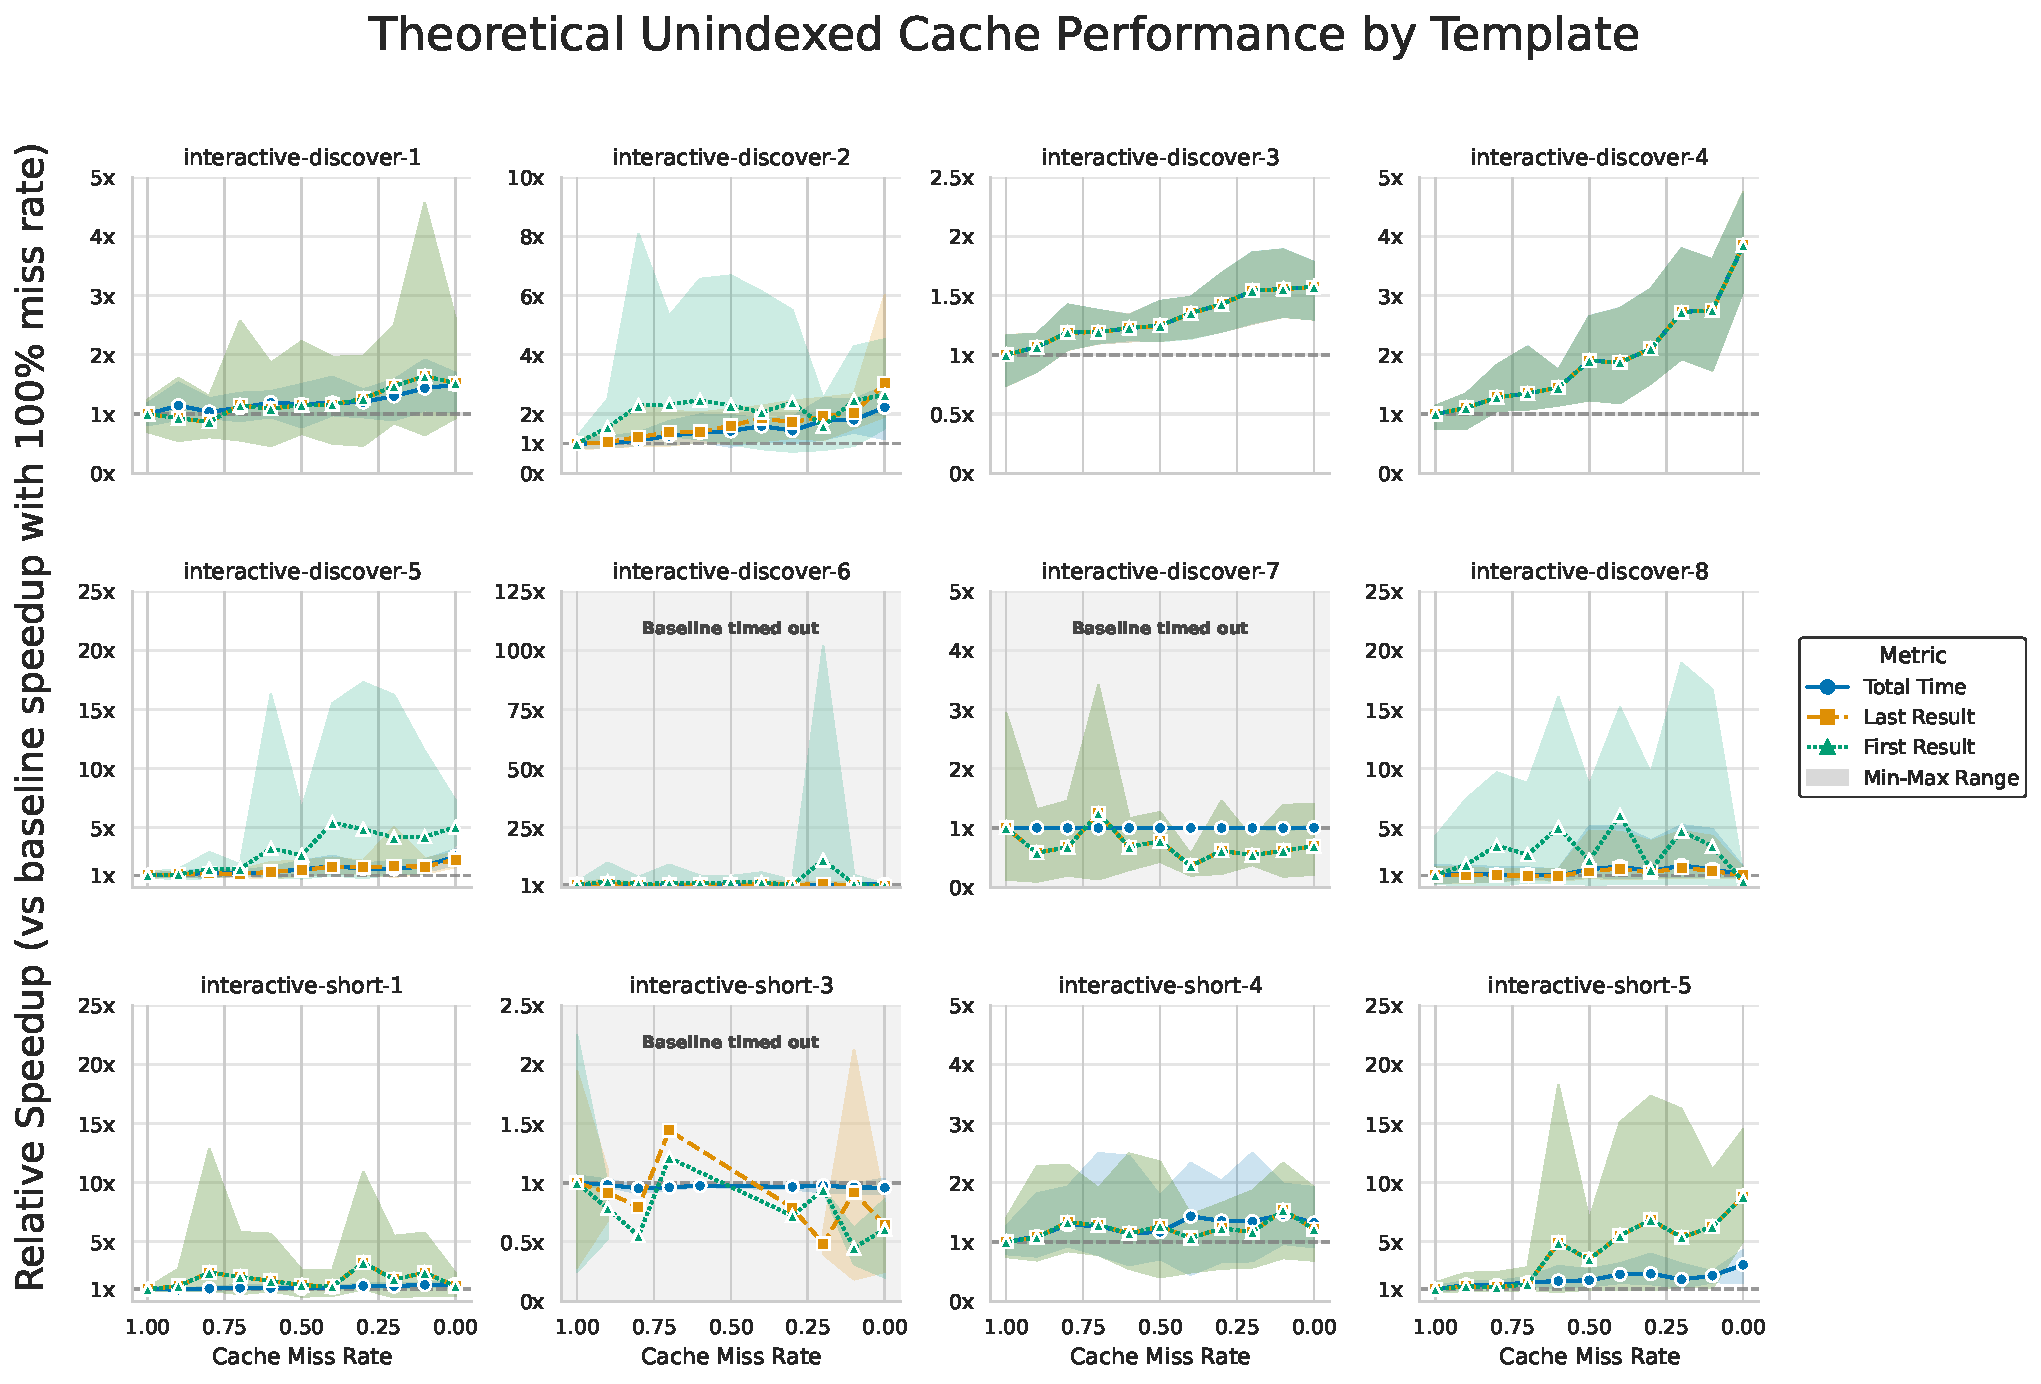
\includegraphics[width=\textwidth]{figures/cache_performance_trellis_academic.pdf}
    \caption{Theoretical unindexed cache performance by query template. Lines indicate the mean relative speedup of the repeated query for total execution time, first result, and last result against a $100\%$ miss rate baseline. Shaded regions denote the absolute minimum and maximum variance across iterations.}
    \label{fig:theoretical_cache_performance}
\end{figure*}

% ---- Bibliography ----
%
% BibTeX users should specify bibliography style 'splncs04'.
% References will then be sorted and formatted in the correct style.
%
% \bibliographystyle{splncs04}
% \bibliography{mybibliography}
%
\bibliographystyle{splncs04}
\bibliography{references/bib}

\end{document}
